%!TEX root = ./slide.tex
%%%%%%%%%%%%%%%%%%%%%%%%%%%%%%%%%%%%%%%%%%%%%%%%%%%%%%%%%%%%%%
% 第２章　非線形システムの線形化
%%%%%%%%%%%%%%%%%%%%%%%%%%%%%%%%%%%%%%%%%%%%%%%%%%%%%%%%%%%%%%

%%%%%%%%%%%%%%%%%%%%%%%%%%%%%%%%%%%%%%%%%%%%%%%%%%%%%%%%%%%%%%
\begin{frame}[t]
\frametitle{2.1 線形システムと非線形システム}
%-------------------------------------------------------------
システムの状態方程式が
\begin{align}
 \frac{dx}{dt} &= A x(t) + B u(t) \tag{\ref{state_eq}} \\
 y(t) &= C x(t) + D u(t) \tag{\ref{output_eq}}
\end{align}
と表されることを前提に制御理論を展開してきた．\\
このシステムは\Blue{\bf {線形システム} (linear system)}であり，理論展開は容易．\\
しかし，実際のシステムには直接は線形状態方程式で表せない\Blue{\bf {非線形システム} (nonlinear system)}が多い．

非線形システム(実システム)に対して線形システム理論を適用するためには，
なんらかの方法で非線形システムを線形化し，線形システムとして扱う必要があ
る．

ここでは，\Blue{非線形システムを線形システムに近似・変換する方法}について説明する．
\end{frame}

%%%%%%%%%%%%%%%%%%%%%%%%%%%%%%%%%%%%%%%%%%%%%%%%%%%%%%%%%%%%%%
\begin{frame}[t]
\frametitle{2.1 線形システムと非線形システム}
%-------------------------------------------------------------
次の非線形状態方程式で表わされる$m$入力$p$出力$n$次のシステムを扱う．
\begin{align}
 \frac{dx}{dt} &= f(x) + g(x) u \label{orsys_state} \\
 y             &= h(x) \label{orsys_output}
\end{align}
ここで\\
\hspace*{1cm}
$x=(x_1, x_2, \cdots, x_n)^T$は状態で$n$次元の縦ベクトル，\\
\hspace*{1cm}
$u=(u_1, u_2, \cdots, u_m)^T$は入力で$m$次元の縦ベクトル，\\
\hspace*{1cm}
$y=(y_1, y_2, \cdots, y_p)^T$は出力で$p$次元の縦ベクトル\\
である．また\\
\hspace*{1cm}
$f(x)$ は$n$次の縦ベクトル値関数，\\
\hspace*{1cm}
$g(x)$ は$n \times m$ の行列値関数，\\
\hspace*{1cm}
$h(x)$ は$p$次の縦ベクトル値関数\\
であり，
その要素は$x$に関して何回でも偏微分可能（$C^\infty$）であり，\\
$f(0) = 0$, $h(0)= 0$
と仮定する．

\end{frame}

%%%%%%%%%%%%%%%%%%%%%%%%%%%%%%%%%%%%%%%%%%%%%%%%%%%%%%%%%%%%%%
\begin{frame}[t]
\frametitle{2.1 線形システムと非線形システム}
%-------------------------------------------------------------
次の非線形状態方程式で表わされる$m$入力$p$出力$n$次のシステムを扱う．
\begin{align}
 \frac{dx}{dt} &= f(x) + g(x) u \tag{\ref{orsys_state}} \\
 y             &= h(x) \tag{\ref{orsys_output}}
\end{align}

線形システムが状態方程式
\begin{align}
	\frac{dx}{dt} & =  A x  + B u \\
	y & =  C x
\end{align}
で表されることを考えれば$f(x)$は$Ax$に，$g(x)$は$B$に，$h(x)$は$Cx$に当たることが容易にわかる．\\
非線形状態方程式(\ref{orsys_state})(\ref{orsys_output})ではバックラッシュや静摩擦，動摩擦，ヒステリシス等を表わすことはできないが，これらの非線形性を無視した機械系の運動方程式などを表わすことができる．
\end{frame}

%%%%%%%%%%%%%%%%%%%%%%%%%%%%%%%%%%%%%%%%%%%%%%%%%%%%%%%%%%%%%%
\begin{frame}[t]
\frametitle{2.1 線形システムと非線形システム}
%-------------------------------------------------------------
例としてFig.~\ref{fig_1_link}に示す簡単なリンク系を考える．
\begin{columns}[t]
\begin{column}{0.55\textwidth}
ここで\\
$\theta$ : リンクの姿勢角（\Blue{システムの出力}）\\
$\dot{\theta} = \frac{d \theta}{dt}$ : リンクの角速度\\
$m$ : リンクの質量，\\
$L$ : 回転軸からリンクの重心までの距離\\
$J$ : リンクの回転軸回りの慣性モーメント\\
$c$ : 回転軸の粘性摩擦係数を\\
$\tau$ : リンクのトルク（\Blue{システムの入力}）\\
$g$ : 重力加速度\\
とすればこのシステムの運動方程式は
\begin{align}
	J \ddot{\theta} &=  -c \dot{\theta} 
				+ m L g \sin \theta 
				+ \tau
\label{link_dynamics}
\end{align}
で表わされる（ただし$\ddot{\theta} = \frac{d^2 \theta}{dt^2}$）．
\end{column}
\begin{column}{0.05\textwidth} 
\end{column}
\begin{column}{0.4\textwidth}
\begin{figure}
	\begin{center}
	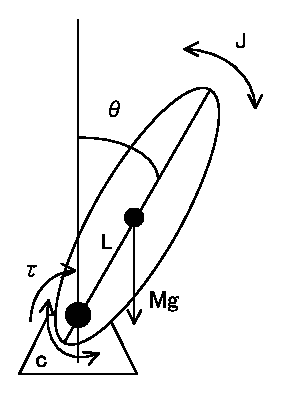
\includegraphics[scale=1.0]{figure/1link.eps}
	\end{center}
	\caption{1リンク系
		 \label{fig_1_link}}
\end{figure}
\end{column}
\end{columns}



\end{frame}

%%%%%%%%%%%%%%%%%%%%%%%%%%%%%%%%%%%%%%%%%%%%%%%%%%%%%%%%%%%%%%
\begin{frame}[t]
\frametitle{2.1 線形システムと非線形システム}
%-------------------------------------------------------------
システムの運動方程式
\begin{align}
	J \ddot{\theta} &=  -c \dot{\theta} 
				+ m L g \sin \theta 
				+ \tau
\tag{\ref{link_dynamics}}
\end{align}

機械系の定石として状態を
\begin{align}
	x&
	=	\left(\begin{array}{c} 
			\mbox{位置・角度} \\ 
			\mbox{速度・角速度}
		\end{array}\right)
	=	\left(\begin{array}{c} 
			\theta \\ 
			\dot{\theta} 
		\end{array}\right)
\end{align}
とすれば，(\ref{link_dynamics})を用いて状態方程式
\begin{align}
	\frac{d}{dt} \left(\begin{array}{c} 
			\theta \\ 
			\dot{\theta} 
		      \end{array}\right)
			&=  \left(\begin{array}{c}
				\dot{\theta} \\
				- \frac{c}{J} \dot{\theta}
				+ \frac{m L g}{J} \sin \theta 
 			      \end{array}\right)
				+ \left(\begin{array}{c}
					0 \\
					\frac{1}{J}
				  \end{array}\right)
				  \tau
\label{link_orsys}
\end{align}
を得る．
\end{frame}

%%%%%%%%%%%%%%%%%%%%%%%%%%%%%%%%%%%%%%%%%%%%%%%%%%%%%%%%%%%%%%
\begin{frame}[t]
\frametitle{2.1 線形システムと非線形システム}
%-------------------------------------------------------------
状態方程式
\begin{align}
	\frac{d}{dt} \left(\begin{array}{c} 
			\theta \\ 
			\dot{\theta} 
		      \end{array}\right)
			&=  \left(\begin{array}{c}
				\dot{\theta} \\
				- \frac{c}{J} \dot{\theta}
				+ \frac{m L g}{J} \sin \theta 
 			      \end{array}\right)
				+ \left(\begin{array}{c}
					0 \\
					\frac{1}{J}
				  \end{array}\right)
				  \tau
	\tag{\ref{link_orsys}}
\end{align}
に対して，
状態$x_L$，入力$u_L$，出力$y_L$を
\begin{align}
	x_L &= \left(\begin{array}{c} 
			x_{L1} \\
			x_{L2} 
		   \end{array}\right) 
			= \left(\begin{array}{c} 
					\theta \\ 
					\dot{\theta} 
			 	\end{array}\right)
,\hspace{5mm}
	u_L = \tau
,\hspace{5mm}
	y_L= \theta
\end{align}
と定義し，さらに$f_L(x_L)$, $g_L(x_L)$, $h_L(x_L)$を
\begin{align}
	f_L(x_L) 
		& =  \left(\begin{array}{c} 
				f_{L1}(x_L) \\
				f_{L2}(x_L) 
			   \end{array}\right) 
		  =  \left(\begin{array}{c}
				x_{L2} \\
				- \frac{c}{J} x_{L2}
					+ \frac{m L g}{J} \sin x_{L1}
		 	   \end{array}\right)
\\
	g_L(x_L) 
		& =  \left(\begin{array}{c} 
				g_{L1}(x_L) \\
				g_{L2}(x_L) 
			   \end{array}\right) 
		  =   \left(\begin{array}{c}
				0 \\
				\frac{1}{J}
			   \end{array}\right)
\\
	h_L(x_L)
		& = x_{L1}
\end{align}
と定義すれば
\end{frame}

%%%%%%%%%%%%%%%%%%%%%%%%%%%%%%%%%%%%%%%%%%%%%%%%%%%%%%%%%%%%%%
\begin{frame}[t]
\frametitle{2.1 線形システムと非線形システム}
%-------------------------------------------------------------
状態方程式
\begin{align}
	\frac{d}{dt} \left(\begin{array}{c} 
			\theta \\ 
			\dot{\theta} 
		      \end{array}\right)
			&=  \left(\begin{array}{c}
				\dot{\theta} \\
				- \frac{c}{J} \dot{\theta}
				+ \frac{m L g}{J} \sin \theta 
 			      \end{array}\right)
				+ \left(\begin{array}{c}
					0 \\
					\frac{1}{J}
				  \end{array}\right)
				  \tau
	\tag{\ref{link_orsys}}
\end{align}
は
\begin{align}
\frac{dx_L}{dt} &= f_L(x_L) + g_L(x_L) u_L 
\\
	y_L &= h_L(x_L)
\label{link_state}
\end{align}
となり，
\begin{align}
 \frac{dx}{dt} &= f(x) + g(x) u \tag{\ref{orsys_state}} \\
 y             &= h(x) \tag{\ref{orsys_output}}
\end{align}
の形の非線形状態方程式で表わされていることがわかる．
\end{frame}

%%%%%%%%%%%%%%%%%%%%%%%%%%%%%%%%%%%%%%%%%%%%%%%%%%%%%%%%%%%%%%
\begin{frame}[t]
\frametitle{2.1 線形システムと非線形システム(線形化)}
%-------------------------------------------------------------
非線形システムの線形化問題のイメージ$\Longrightarrow$\\
Fig.\ref{fig:nonlinimage}の曲線を\Blue{如何にFig.\ref{fig:linimage}の直線に変形するか}(または近似するか)

\begin{figure}[htbp]
 \renewcommand{\subcapsize}{\normalsize}
 \def\subfigcapskip{0pt}
  \begin{center}
    \subfigure[線形システムのイメージ]{%
    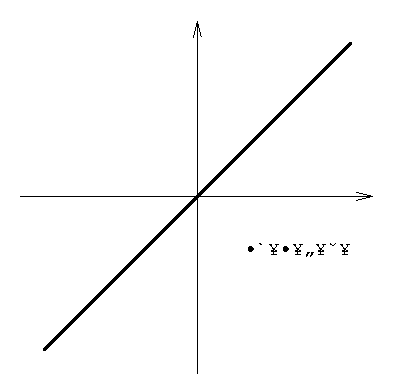
\epsfig{file=figure/linimage.eps,scale=0.8}
    \label{fig:linimage}
    } \hspace{5mm}
    \subfigure[非線形システムのイメージ]{%
    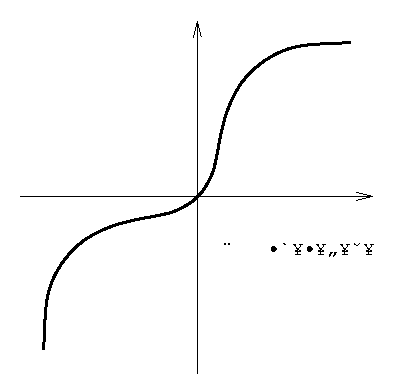
\epsfig{file=figure/nonlinimage.eps,scale=0.8}
    \label{fig:nonlinimage}
    }
   \caption{システムのイメージ}
  \end{center}
\end{figure}
\end{frame}

%%%%%%%%%%%%%%%%%%%%%%%%%%%%%%%%%%%%%%%%%%%%%%%%%%%%%%%%%%%%%%
\begin{frame}[t]
\frametitle{2.2 テーラー展開の1次近似線形化}
%-------------------------------------------------------------
一般的な線形化手法は\Blue{テーラー展開の１次近似}に基づいたものである．\\
非線形状態方程式
\begin{align}
 \frac{dx}{dt} &= f(x) + g(x) u \tag{\ref{orsys_state}} \\
 y             &= h(x) \tag{\ref{orsys_output}}
\end{align}
において$x=0$, $u=0$
が平衡点($\frac{dx}{dt} = 0$となり，状態$x$が変化しない点)であることに注
意して，この平衡点のまわりで(\ref{orsys_state})の右辺をテーラー展開し，
１次の近似を行えば次の式を得る．
\end{frame}

%%%%%%%%%%%%%%%%%%%%%%%%%%%%%%%%%%%%%%%%%%%%%%%%%%%%%%%%%%%%%%
\begin{frame}[t]
\frametitle{2.2 テーラー展開の1次近似線形化}
%-------------------------------------------------------------
\begin{align}
 \frac{dx}{dt} 
 &= f(0) + \left. \frac{\partial f}{\partial x} \right \vert _{x=0} x
 + g(0) u + O^2 (x, u) \nonumber \\
 &= \left. \frac{\partial f}{\partial x} \right \vert _{x=0} x
 + g(0) u + O^2 (x, u)
 \label{app1_state_p}
\\
 y 
 &= h(0) + \left. \frac{\partial h}{\partial x} \right \vert _{x=0} x
 + O^2 (x, u)
 \nonumber \\
 &= \left. \frac{\partial h}{\partial x} \right \vert _{x=0} x
 + O^2 (x, u)
\end{align}
ここで$O^2(x, u)$は$x$と$u$に関して2次以上の項を表わす．
\end{frame}

%%%%%%%%%%%%%%%%%%%%%%%%%%%%%%%%%%%%%%%%%%%%%%%%%%%%%%%%%%%%%%
\begin{frame}[t]
\frametitle{2.2 テーラー展開の1次近似線形化}
%-------------------------------------------------------------
また
$x = (x_1, x_2, \cdots, x_n)^T$, $q(x) = (q_1(x), q_2(x), \cdots,
q_r(x))^T$とするとき
\begin{equation}
 \frac{\partial q}{\partial x} = 
  \left(\begin{array}{cccc}
   \frac{\partial q_1}{\partial x_1} &
    \frac{\partial q_1}{\partial x_2} &
    \cdots &
    \frac{\partial q_1}{\partial x_n} \\
	 \frac{\partial q_2}{\partial x_1} &
	  \frac{\partial q_2}{\partial x_2} &
	  \cdots &
	  \frac{\partial q_2}{\partial x_n} \\
	 \vdots & \vdots & & \vdots \\
	 \frac{\partial q_r}{\partial x_1} &
	  \frac{\partial q_r}{\partial x_2} &
	  \cdots &
	  \frac{\partial q_r}{\partial x_n}
	\end{array}\right)
\end{equation}
$
  \left(\begin{array}{c}
	f_1(x_1,x_2) \\
	f_2(x_1,x_2) 
  \end{array}\right)
$
の原点周りの1次のテーラー展開は
\begin{align*}
  \left(\begin{array}{c}
	f_1(x_1,x_2) \\
	f_2(x_1,x_2) 
  \end{array}\right)
  &=
  \left(\begin{array}{c}
	f_1(0,0) +
	\left[ \frac{\partial f_1}{\partial x_1} \right]_{x=0} x_1 
	   + \left[ \frac{\partial f_1}{\partial x_2} \right]_{x=0} x_2 \\
	f_2(0,0) +
	\left[ \frac{\partial f_2}{\partial x_1}\right]_{x=0} x_1 
		+ \left[ \frac{\partial f_2}{\partial x_2}\right]_{x=0} x_2
  \end{array}\right)
  + O^2(x_1,x_2)
  \nonumber \\
  &=
  \left(\begin{array}{c}
	f_1(0,0) \\
	f_2(0,0) 
  \end{array}\right)
  +
  \left(\begin{array}{cc}
	\frac{\partial f_1}{\partial x_1}
		& \frac{\partial f_1}{\partial x_2} \\
	\frac{\partial f_2}{\partial x_1}
		& \frac{\partial f_2}{\partial x_2}
  \end{array}\right)_{x=0}
  \left(\begin{array}{c}
	x_1 \\
	x_2 
  \end{array}\right)
  + O^2(x_1,x_2)
\end{align*}
\end{frame}

%%%%%%%%%%%%%%%%%%%%%%%%%%%%%%%%%%%%%%%%%%%%%%%%%%%%%%%%%%%%%%
\begin{frame}[t]
\frametitle{2.2 テーラー展開の1次近似線形化}
%-------------------------------------------------------------
$\left. \frac{\partial f}{\partial x} \right \vert _{x=0}$, $
g(0)$, $\left. \frac{\partial h}{\partial x} \right \vert _{x=0}$は既に定数となっていることから
\begin{equation}
 A \defeq \left.\frac{\partial f}{\partial x} \right \vert _{x=0},
  \quad	B \defeq g(0),
  \quad	C \defeq \left. \frac{\partial h}{\partial x} \right \vert _{x=0}
\end{equation}
と定義し，また(\ref{app1_state_p})において$x$と$u$が十分小さいとして$
O^2(x, u)$の項を無視すれば，テーラー展開の１次近似として以下の線形シ
ステムを得る．
\begin{align}
 \frac{dx}{dt} &= A x + B u
  \label{first_approx}
\\
 y&= C x
\end{align}
\end{frame}

%%%%%%%%%%%%%%%%%%%%%%%%%%%%%%%%%%%%%%%%%%%%%%%%%%%%%%%%%%%%%%
\begin{frame}[t]
\frametitle{2.2 テーラー展開の1次近似線形化}
%-------------------------------------------------------------
\addtocounter{equation}{-2}
線形化されたシステム
\begin{align}
 \frac{dx}{dt} &= A x + B u
\\
 y&= C x
\end{align}
に対する
コントローラーの設計は，この近似線形化されたシステムに対して線形制御理論を
用いて行えばよい．例えば状態フィードバックを用いるならば
\begin{equation}
 u = Fx
\end{equation}
となり，コントローラーは線形である．

\end{frame}

%%%%%%%%%%%%%%%%%%%%%%%%%%%%%%%%%%%%%%%%%%%%%%%%%%%%%%%%%%%%%%
\begin{frame}[t]
\frametitle{2.2 テーラー展開の1次近似線形化}
%-------------------------------------------------------------
この線形化はイメージ的にはFig.\ref{image_taylor_linearization}に示すように，
元の曲線(非線形システム)に対して原点の近くで接線を引き，
この接線を近似線形化されたシステムと考えることに相当する．\\
\begin{itemize}
	\item 原点から離れると近似が悪くなる\\
	$\Longrightarrow$ \Red{原点の近くでしか有効でないことが多い}
	\item 手法が簡潔で\Blue{ほとんどすべてのシステムに対して適用可能}
\end{itemize}
\vspace*{-5mm}

\begin{columns}[t]
\begin{column}{0.55\textwidth}
\begin{figure}[htbp]
 \begin{center}
  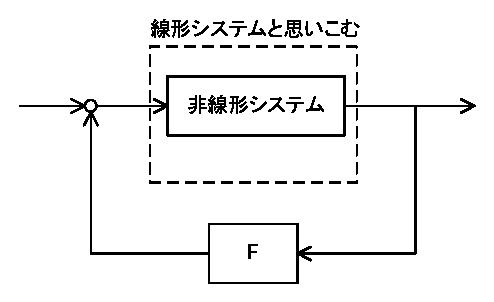
\epsfig{file=figure/taylorblock.eps,scale=0.8}
  \caption{テーラー展開の一次近似線形化を用いた制御系}
  \label{block_taylor_linearization}
 \end{center}
\end{figure}
\end{column}
\begin{column}{0.05\textwidth} 
\end{column}
\begin{column}{0.4\textwidth}
\begin{figure}[htbp]
 \begin{center}
  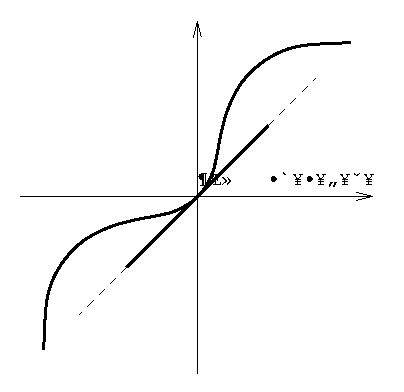
\epsfig{file=figure/taylorimage.eps,scale=0.6}
  \caption{テーラー展開の１次近似線形化のイメージ}
  \label{image_taylor_linearization}
 \end{center}
\end{figure}
\end{column}
\end{columns}
\end{frame}

%%%%%%%%%%%%%%%%%%%%%%%%%%%%%%%%%%%%%%%%%%%%%%%%%%%%%%%%%%%%%%
\begin{frame}[t]
\frametitle{2.3 非線形フィードバックによる厳密な線形化}
%-------------------------------------------------------------
近似線形化は平衡点(ここでは原点)の近くでの近似線形化でしかなく，そのため，
近似の精度も必ずしも十分ではないことがある．\\
$\Longrightarrow$ ロボットのように作業範囲が大きく，かつ非線形性の大きなシステムに対しては\Red{利用できない}ことがある．\\
そのため，ロボット工学の分野ではこれと異なった線形化(近似ではなく\Blue{厳密な線形化})が行なわれるようになった．これは状態$x$が利用可能な場合に利用可能となる．
\end{frame}

%%%%%%%%%%%%%%%%%%%%%%%%%%%%%%%%%%%%%%%%%%%%%%%%%%%%%%%%%%%%%%
\begin{frame}[t]
\frametitle{2.3 非線形フィードバックによる厳密な線形化}
%-------------------------------------------------------------
ロボットなどの機械系の場合は，運動方程式が特殊な形をしていることが多い．例
えば多くのロボットの運動方程式は
\begin{equation}
 M(\theta) \ddot{\theta} + k(\theta, \dot{\theta}) = \tau
  \label{2_link_robot}
\end{equation}
で表わされることが知られている．\\
ここで\\
$\theta$ : ロボットの姿勢角，\\
$M(\theta)$ : は慣性モーメント($\theta$の関数であり一般には常に正則)\\
$k(\theta, \dot{\theta})$ : 遠心力やコリオリ力を表わす項\\
$\tau$は各リンクへのトルク入力\\
である．
\end{frame}

%%%%%%%%%%%%%%%%%%%%%%%%%%%%%%%%%%%%%%%%%%%%%%%%%%%%%%%%%%%%%%
\begin{frame}[t]
\frametitle{2.3 非線形フィードバックによる厳密な線形化}
%-------------------------------------------------------------
さて$M(\theta)$が正則であることから,ロボットの運動方程式
\begin{equation}
 M(\theta) \ddot{\theta} + k(\theta, \dot{\theta}) = \tau
  \tag{\ref{2_link_robot}}
\end{equation}
に対してフィードバック
\begin{equation}
 \tau = k(\theta,\dot{\theta}) + M(\theta) v 
\end{equation}
を用いる($v$は新しい入力)と
\begin{equation}
 \ddot{\theta} = v 
\end{equation}
となる．\\
これを状態方程式で表わせば
\begin{equation}
 \frac{d}{dt}
  \left(\begin{array}{c}
   \theta \\
	 \dot{\theta}
	\end{array}\right)
  =
  \left(\begin{array}{cc}
   0 & I \\
	 0 & 0 
	\end{array}\right)
  \left(\begin{array}{c}
   \theta \\
	 \dot{\theta}
	\end{array}\right)
  +
  \left(\begin{array}{c}
   0 \\
	 I
	\end{array}\right)
  v
  \label{robot_linearized_sys}
\end{equation}
のように，状態を$(\theta^T, \dot{\theta}^T)^T$，入力を$v$とした線形状態方
程式となる．\\
この線形化された状態方程式に対して線形制御理論を用いてコント
ローラーを設計すれば，$\theta$を容易に制御することができる．
\end{frame}

%%%%%%%%%%%%%%%%%%%%%%%%%%%%%%%%%%%%%%%%%%%%%%%%%%%%%%%%%%%%%%
\begin{frame}[t]
\frametitle{2.3 非線形フィードバックによる厳密な線形化}
%-------------------------------------------------------------
厳密に線形化されたシステム
\begin{equation}
 \frac{d}{dt}
  \left(\begin{array}{c}
   \theta \\
	 \dot{\theta}
	\end{array}\right)
  =
  \left(\begin{array}{cc}
   0 & I \\
	 0 & 0 
	\end{array}\right)
  \left(\begin{array}{c}
   \theta \\
	 \dot{\theta}
	\end{array}\right)
  +
  \left(\begin{array}{c}
   0 \\
	 I
	\end{array}\right)
  v
  \tag{\ref{robot_linearized_sys}}
\end{equation}
を安定化するコントローラーとして状態フィードバック
\begin{equation}
 v = F
  \left(\begin{array}{c}
   \theta \\
	 \dot{\theta}
	\end{array}\right)
\end{equation}
を用いれば，元のシステム
\begin{equation}
 M(\theta) \ddot{\theta} + k(\theta, \dot{\theta}) = \tau
  \tag{\ref{2_link_robot}}
\end{equation}
に対するコントローラーは
\begin{equation}
 \tau = k(\theta, \dot{\theta}) + M(\theta) F
  \left(\begin{array}{c}
   \theta \\
	 \dot{\theta}
	\end{array}\right)
\end{equation}
となる．このときのコントローラーは前節と異なり，非線形であることに注意する．
この制御系の様子をFig.\ref{config_nonlinear_feedback}に示す．
\end{frame}

%%%%%%%%%%%%%%%%%%%%%%%%%%%%%%%%%%%%%%%%%%%%%%%%%%%%%%%%%%%%%%
\begin{frame}[t]
\frametitle{2.3 非線形フィードバックによる厳密な線形化}
%-------------------------------------------------------------
この線形化のイメージはFig.\ref{image_lin_w_fb}のように元の曲線(非線形システム)を入
力を使って強制的に直線(線形システム)にするものである．
\vspace{-5mm}
\begin{columns}[t]
\begin{column}{0.55\textwidth}
\begin{figure}[htbp]
 \begin{center}
	\scalebox{.6}{ 
  	\input{../figure/nonlinfeedbackblock.pstex_t}
  }
  \caption{非線形フィードバックによる線形化を用いた制御系}
  \label{config_nonlinear_feedback}
 \end{center}
\end{figure}
\end{column}
\begin{column}{0.4\textwidth}
\vspace{10mm}
\begin{figure}[htbp]
 \begin{center}
  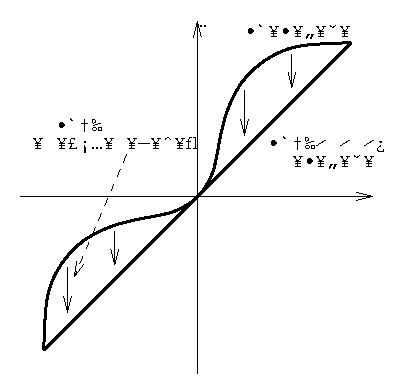
\epsfig{file=../figure/exactimage.eps,scale=0.6}
  \caption{非線形フィードバックを用いた線形化のイメージ}
  \label{image_lin_w_fb}
 \end{center}
\end{figure}
\end{column}
\end{columns}
\end{frame}

%%%%%%%%%%%%%%%%%%%%%%%%%%%%%%%%%%%%%%%%%%%%%%%%%%%%%%%%%%%%%%
\begin{frame}[t]
\frametitle{2.3 非線形フィードバックによる厳密な線形化}
%-------------------------------------------------------------
この線形化は近似を用いない厳密な線形化であるため，線形化されたシステムを
用いて設計されたコントローラーは\Blue{原点の近くのみでなく，状態全体で有効となる}．

この方法は直感的であるため，ダイナミクスが
\begin{equation}
 M(\theta,\dot{\theta}, \cdots \theta^{(r-1)}) \theta^{(r)} 
  + k(\theta,\dot{\theta}, \cdots \theta^{(r-1)}) 
  = N(\theta,\dot{\theta}, \cdots \theta^{(r-1)}) u
  \label{linearizable_with_feedback}
\end{equation}
で表わされるシステムにしか応用できない．\\
(ここで$\theta^{(i)} =\frac{d^{i} \theta}{dt^i}$とし，$M(\cdot)$と$N(\cdot)$は常に正則とする．)\\
しかし，機械系などのように(\ref{linearizable_with_feedback})で表わされる
システムが多いことも事実である．
\end{frame}

%%%%%%%%%%%%%%%%%%%%%%%%%%%%%%%%%%%%%%%%%%%%%%%%%%%%%%%%%%%%%%
\begin{frame}[t]
\frametitle{2.4 座標変換と非線形フィードバックを用いた
%-------------------------------------------------------------
\\厳密な線形化}
\begin{itemize}
	\item テーラー展開の１次近似を用いた線形化:\\
	システムの線形近似であり，狭い範囲でしか有効でない．
	\item 線形化は厳密な線形化:\\
	特殊な形をしたシステムにしか適用可能でない．
\end{itemize}

ここから状態方程式
\begin{align}
 \frac{dx}{dt} &= f(x) + g(x) u \tag{\ref{orsys_state}}
\end{align}
で表わされたシステムに対して，
非線形フィードバックのみでなく\Blue{座標変換まで用いて厳密に線形化する方法}について説明する．\\
この線形化について
\begin{itemize}
	\item システムが線形化されるための必要十分条件
	\item システムを線形化する座標変換と非線形フィードバックの求め方
\end{itemize}
が非線形システム理論(幾何学的アプローチ)により得られている
が本講義では省略し，概要のみを説明する．
\end{frame}

%%%%%%%%%%%%%%%%%%%%%%%%%%%%%%%%%%%%%%%%%%%%%%%%%%%%%%%%%%%%%%
\begin{frame}[t]
\frametitle{2.4 座標変換と非線形フィードバックを用いた\\
厳密な線形化}
%-------------------------------------------------------------
ここでは状態$x$が利用可能であると仮定する．
システム
\begin{align}
 \frac{dx}{dt} &= f(x) + g(x) u \tag{\ref{orsys_state}}
 \end{align}
に対して次の座標変換とフィードバックを考える
($v$は新しい入力)．
\begin{align}
 \xi &= T(x) \label{cord} \\
 u   &= \alpha (x) + \beta (x) v
  \label{feedback}
\end{align}
ここで$T(x)$は原点を原点に変換する($T(0)=0$)と仮定する．\\
これにより状態
方程式(\ref{orsys_state})は以下となる．
\begin{align}
 \frac{d \xi}{dt} 
  &= \frac{\partial \xi}{\partial x} \frac{dx}{dt} \nonumber \\
 &= \frac{\partial T}{\partial x} 
  \{ f(T^{-1}(\xi)) + g(T^{-1}(\xi)) \alpha(T^{-1}(\xi)) \}
  + \frac{\partial T}{\partial x} g(T^{-1}(\xi)) \beta (T^{-1}(\xi)) v \\
 &\defeq \bar{f}(\xi) + \bar{g}(\xi) v
  \label{feed_state}
\end{align}

\end{frame}

%%%%%%%%%%%%%%%%%%%%%%%%%%%%%%%%%%%%%%%%%%%%%%%%%%%%%%%%%%%%%%
\begin{frame}[t]
\frametitle{2.4 座標変換と非線形フィードバックを用いた\\
厳密な線形化}
%-------------------------------------------------------------
システム
\begin{align}
 \frac{dx}{dt} &= f(x) + g(x) u \tag{\ref{orsys_state}}
 \end{align}
に対して座標変換とフィードバック
\begin{align}
 \xi &= T(x) \tag{\ref{cord}} \\
 u   &= \alpha (x) + \beta (x) v
  \tag{\ref{feedback}}
\end{align}
が施されたシステム
\begin{align}
 \frac{d \xi}{dt} 
 &\defeq \bar{f}(\xi) + \bar{g}(\xi) v
  \tag{\ref{feed_state}}
\end{align}
が
\begin{equation}
 \bar{f}(\xi) = A \xi, \quad \bar{g}(\xi) = B 
  \label{linear}
\end{equation}
かつ$(A, B)$可制御となるように座標変換とフィードバックが求められるならば，
システムを$\xi$座標系で厳密に線形システムと一致させることができる．
この線形化は近似ではなく厳密な線形化である．
\end{frame}

%%%%%%%%%%%%%%%%%%%%%%%%%%%%%%%%%%%%%%%%%%%%%%%%%%%%%%%%%%%%%%
\begin{frame}[t]
\frametitle{2.4 座標変換と非線形フィードバックを用いた\\
厳密な線形化}
%-------------------------------------------------------------
この線形化されたシステム
\begin{align}
 \frac{d \xi}{dt} 
 &\defeq \bar{f}(\xi) + \bar{g}(\xi) v = A\xi + Bv
  \tag{\ref{feed_state}}
\end{align}
に対しては，線形制御理論を用いてコントローラーを設
計することができる．\\
例えば，状態フィードバック
\begin{equation}
 v = F \xi
  \label{linear_feedback}
\end{equation}
を設計すれば，元のシステムに対するコントローラーは次式となる．
\begin{align}
 u &= \alpha(x) + \beta(x) F \xi \nonumber \\
   &= \alpha(x) + \beta(x) F T(x)
    \label{nonlinear_feedback}
\end{align}
座標変換$\xi = T(x)$ が原点を原点に写像することから，
$\xi
\rightarrow 0$ならば$x \rightarrow 0$である．
つまり，線形化されたシステムを安定化するフィードバック(\ref{linear_feedback})に基づいて設計されたフィードバック(\ref{nonlinear_feedback})は元のシステム
\begin{align}
 \frac{dx}{dt} &= f(x) + g(x) u \tag{\ref{orsys_state}}
 \end{align}
 を安定化する．
\end{frame}

%%%%%%%%%%%%%%%%%%%%%%%%%%%%%%%%%%%%%%%%%%%%%%%%%%%%%%%%%%%%%%
\begin{frame}[t]
\frametitle{2.4 座標変換と非線形フィードバックを用いた\\
厳密な線形化}
%-------------------------------------------------------------
\begin{figure}[htbp]
 \begin{center}
 	\scalebox{0.7}{
  	\input{../figure/nonlinfeedbackconvblock.pstex_t}
	}
  \caption{非線形フィードバックと座標変換を用いた線形化による制御系}
  \label{config_lin_w_fd_cor}
 \end{center}
\end{figure}
\end{frame}


%%%%%%%%%%%%%%%%%%%%%%%%%%%%%%%%%%%%%%%%%%%%%%%%%%%%%%%%%%%%%%
\begin{frame}[t]
\frametitle{2.4 座標変換と非線形フィードバックを用いた\\
厳密な線形化}
%-------------------------------------------------------------
この線形化のイメージはFig.\ref{image_lin_w_fb_cor}のように元の曲線(非線形システム)を座標
を変えて直線(線形システム)にすることである．

\begin{figure}[htbp]
 \begin{center}
 	\scalebox{0.7}{
	  \input{../figure/nonlinfeedbackconvimage.pstex_t} % scale = 100%
  }
  \caption{非線形フィードバックと座標変換を用いた線形化のイメージ}
  \label{image_lin_w_fb_cor}
 \end{center}
\end{figure}

\end{frame}

%%%%%%%%%%%%%%%%%%%%%%%%%%%%%%%%%%%%%%%%%%%%%%%%%%%%%%%%%%%%%%%
\begin{frame}[t]
\frametitle{2. 非線形システムの線形化　＜演習＞線形化}
%-------------------------------------------------------------
次の１リンク系の運動方程式を考える．
\[
	J \ddot{\theta} = -c \dot{\theta} + mLg \sin \theta + \tau
\]\nopagebreak
ここで$\theta$はリンク角，$\tau$は入力トルクで，のこりは定数である．

\begin{enumerate}
\item 
このシステムを状態方程式であらわせ．
\item
状態方程式をテーラー展開の１次近似線形化せよ．
\item
運動方程式をフィードバック線形化し，線形状態方程式を求めよ．
\end{enumerate}
\end{frame}



